\documentclass[aspectratio=169]{beamer}
\usetheme{Madrid}

\usepackage{graphicx}
\usepackage[utf8]{inputenc}
\usepackage{hyperref}
\usepackage{listings}
\usepackage{xcolor}
%\usepackage{subfig}
\usepackage{subcaption}

%\setbeamertemplate{footline}[frame number]

\begin{document}

\title{Introduction to Neural Networks}  
\subtitle{Convolutional Neural Networks} 
\author[J.I. Vasquez]{\textbf{Juan Irving Vásquez} \\jivg.org}
\date{\today \copyright}
\institute[jivg.org]{Centro de Innovación y Desarrollo Tecnológico en Cómputo \\ Instituto Politécnico Nacional}
% logo of my university
\titlegraphic{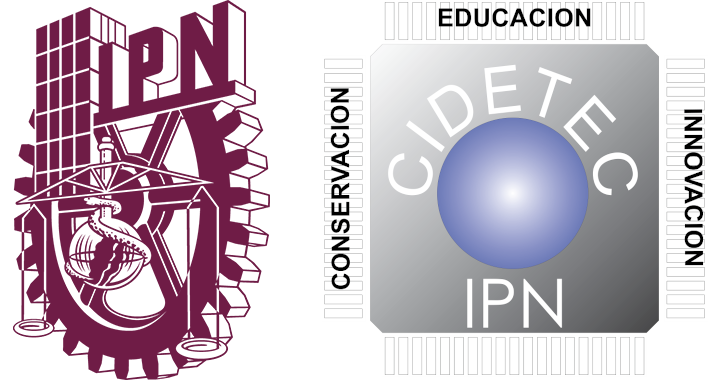
\includegraphics[width=2cm]{ipn-cidetec}}

\frame{\titlepage}


\frame{
	\frametitle{Contents}
	\tableofcontents
}

\AtBeginSection[] { \begin{frame} \frametitle{Roadmap} \tableofcontents[currentsection] \end{frame} }


\section{Motivation}

\begin{frame}
\frametitle{The fully connected networks}
The FCN can be adapted to recognize patterns in several dimensions.
\begin{center}
	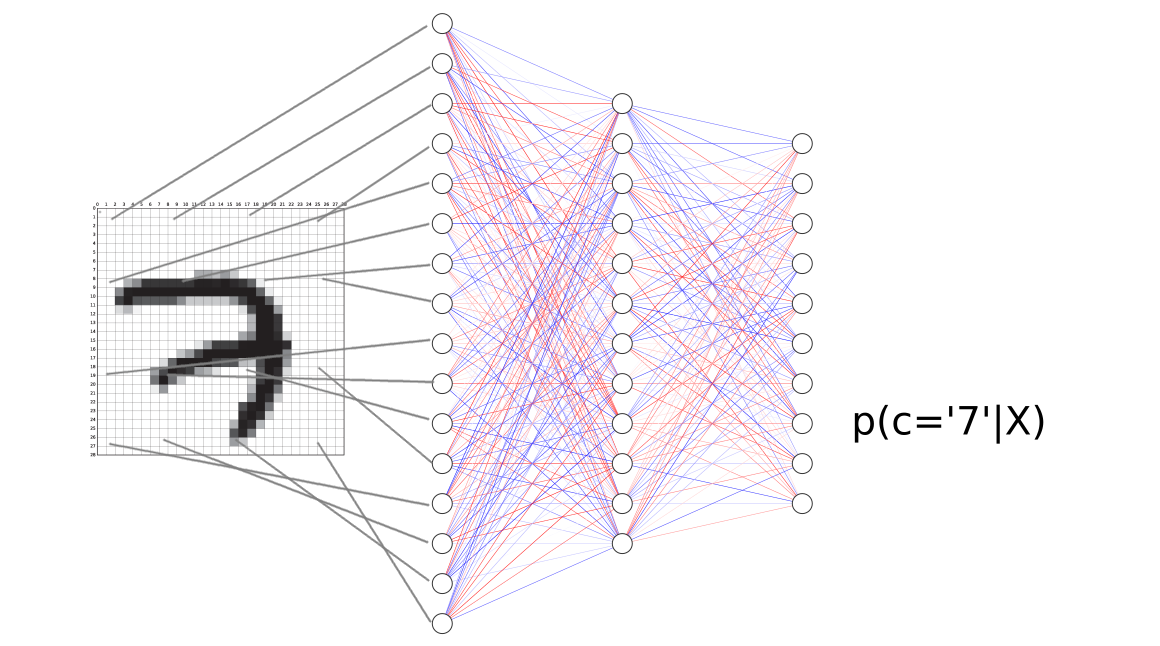
\includegraphics[height=0.55\textheight]{nn7.png}
\end{center}
"The response of most of these models, however, was severely affected by the shift in position and/or by the distortion in shape of the input patterns"\footnote{\tiny Fukushima, Kunihiko. "Neocognitron: A self-organizing neural network model for a mechanism of pattern recognition unaffected by shift in position." Biological cybernetics 36.4 (1980): 193-202.}
\end{frame}

\begin{frame}
\frametitle{Convolutional Neural Networks (CNN)}
\begin{itemize}
	\item Position invariance of features
	\begin{center}
		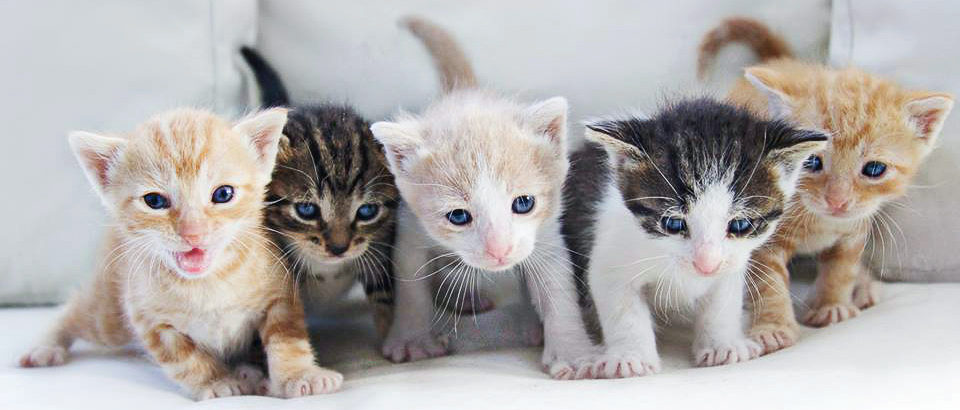
\includegraphics[height=0.6\textheight]{cats}
	\end{center}
	\pause
	\item CNNs share their parameters across the space
\end{itemize}
\end{frame}


\begin{frame}{Template matching}
\begin{itemize}
	\item Template
	\begin{center}
		
\includegraphics[height=0.2\textheight]{cute-cat-face}
	\end{center}
	\item Picture
		\begin{center}
		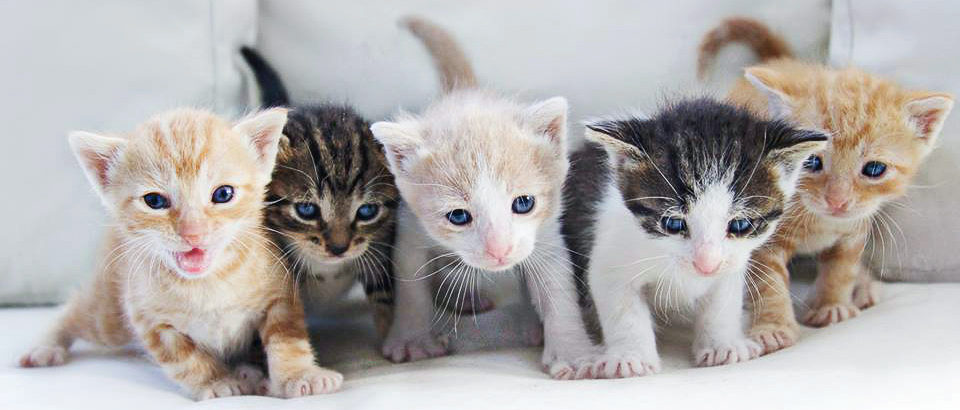
\includegraphics[height=0.4\textheight]{cats}
	\end{center}
\end{itemize}
\end{frame}


\begin{frame}
	\frametitle{Convolution property}
	\framesubtitle{Graphical motivation}
	\begin{figure}
		\begin{subfigure}{.35\textwidth}
			\centering
			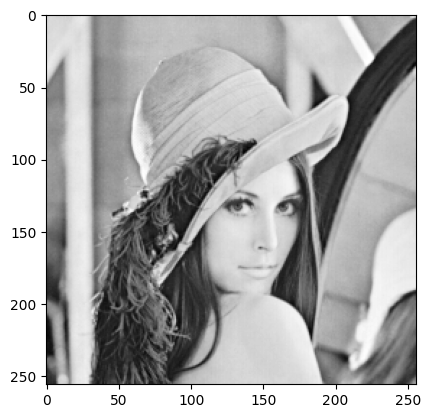
\includegraphics[width=\linewidth]{lenagris.png}
			\caption{Input image (I)}
			\label{fig:sfig1}
		\end{subfigure}%
		\begin{subfigure}{0.25\textwidth}
			$$K = 
			\left[ 
			\begin{matrix}
				-1 & 0 & 1 \\
				-1 & 0 & 1 \\
				-1 & 0 & 1 \\
			\end{matrix}
			\right] $$
			\caption{Kernel}
		\end{subfigure}
		\begin{subfigure}{.35\textwidth}
			\centering
			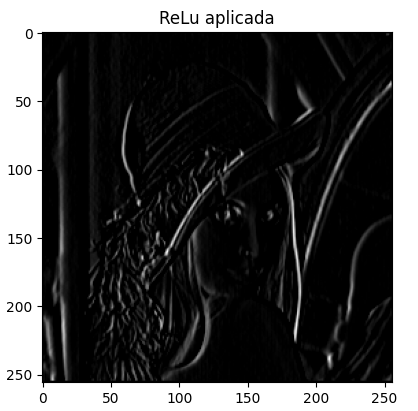
\includegraphics[width=\linewidth]{ccnout.png}
			\caption{Output (G)}
			\label{fig:sfig2}
		\end{subfigure}
		%\caption{Efecto de la convolución sobre una imagen cuando se usa un kernel para detectar bordes verticales. Como se observa en la salida, la convolución resalta aquellos pixeles donde se encuentran bordes verticales que de izquierda a derecha cambian de obscuro a claro.}
		%\label{fig:ej_convolucion}
	\end{figure}
\end{frame}


\begin{frame}
\frametitle{Convolutional Neural Networks insight}
The convolutional neural networks were introduced by LuCun in 1989.
\begin{figure}
	\centering
	\includegraphics[width=0.6\linewidth]{"cnn scheme"}
	\caption{Scheme of a convolutional neural network for classification.}
	\label{fig:cnn-scheme}
\end{figure}
\end{frame}



\section{Bidimensional convolution}


\begin{frame}
	\frametitle{Convolution Inputs}
	\begin{itemize}
		\item Input
		\begin{equation}
			I = \left[ \begin{matrix}
				x_{1,1} & \dots & x_{1,m} \\
				\vdots & \ddots & ·\vdots \\
				x_{m,1} & \dots & x_{l,m} \\
			\end{matrix} \right]
		\end{equation} where $I\in \mathbb{R}^{m\times m}$, y
		\item Kernel
		\begin{equation}
			\textbf{K} = \left[ \begin{matrix}
				w_{1,1} & \dots & w_{1,k} \\
				\vdots & \ddots & ·\vdots \\
				w_{k,1} & \dots & w_{k,k} \\
			\end{matrix} \right]
		\end{equation} where $\textbf{K}\in \mathbb{R}^{k\times k}$, $k = (2l+1)$ y $k < m$. 
	\end{itemize}
\end{frame}


\begin{frame}
\frametitle{2D Discrete Convolution}
\framesubtitle{Mathematical definition}

\begin{itemize}
	\item Given two functions, $I$ and $\textbf{K}$, the convolution produces a new function that changes the shape of the first one according the to second one. 
	\begin{equation}
	G[i,j] =  \sum_{u=-l}^{l} \sum_{v=-l}^{l} \textbf{K}[u,v] I[i-u,j-v]
	\end{equation}
	\item It is very useful to find patterns.
\end{itemize}
\end{frame}


\begin{frame}
	\frametitle{Cross correlation}
	\framesubtitle{In neural networks}
	\begin{itemize}
		\item Given two functions, $I$ and $\textbf{K}$
		\begin{equation}
			G[i,j] =  \sum_{u=-l}^{l} \sum_{v=-l}^{l} \textbf{K}[u,v] I[i+u,j+v]
		\end{equation}
		\item The cross correlation is more used in machine learning.
	\end{itemize}
\end{frame}


\begin{frame}
	\frametitle{Convolution layer}
	\begin{figure}[tb]
		\centering
		% Cada subfigura ocupa ~1/4 del ancho del texto
		\begin{subfigure}[t]{0.24\textwidth}
			\centering
			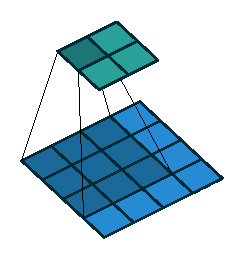
\includegraphics[width=\linewidth]{no_padding_no_strides_00.pdf}
			\caption{Step 1}
			\label{fig:ejemplo:a}
		\end{subfigure}\hfill
		\begin{subfigure}[t]{0.24\textwidth}
			\centering
			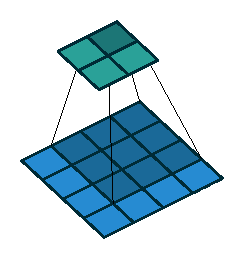
\includegraphics[width=\linewidth]{no_padding_no_strides_01.pdf}
			\caption{Step 2}
			\label{fig:ejemplo:b}
		\end{subfigure}\hfill
		\begin{subfigure}[t]{0.24\textwidth}
			\centering
			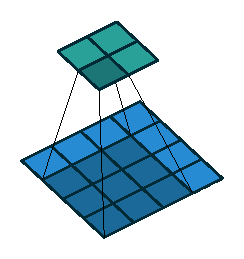
\includegraphics[width=\linewidth]{no_padding_no_strides_02.pdf}
			\caption{Step 3}
			\label{fig:ejemplo:c}
		\end{subfigure}\hfill
		\begin{subfigure}[t]{0.24\textwidth}
			\centering
			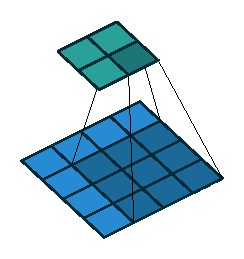
\includegraphics[width=\linewidth]{no_padding_no_strides_03.pdf}
			\caption{Step 4}
			\label{fig:ejemplo:d}
		\end{subfigure}
		\caption{Convolution: a kernel is moved inside the input to create a new matrix.}
		\label{fig:filter}
	\end{figure}
%	\begin{figure}
%		\centering
%		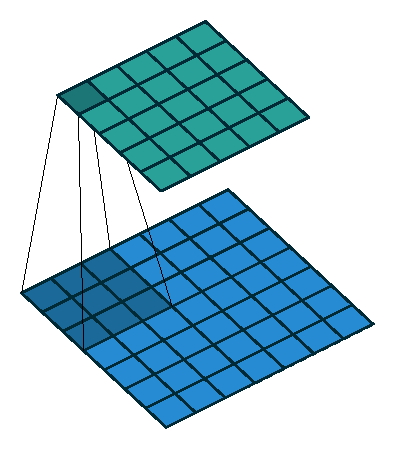
\includegraphics[height=0.6\textheight]{full_padding_no_strides_transposed_00}
%		\caption{Convolution: a kernel is moved inside the input to create a new matrix.}
%		\label{fig:filter}
%	\end{figure}
	{\scriptsize  \url{https://github.com/vdumoulin/conv_arithmetic/raw/master/gif/no_padding_no_strides.gif}{} }
\end{frame}



\begin{frame}
	\frametitle{Convolutional layer}
	Composed by:
	\begin{itemize}
		\item Convolution \footnote{Similar to Pytorch Conv2D}
			\begin{equation}
			\texttt{Conv2D}(K,I)[i,j] = b + \sum_{u=-l}^{l} \sum_{v=-l}^{l} \textbf{K}[u,v] I[i+u,j+v]
			\label{eq:conv2d}
		\end{equation}
		
		\item Activation
		    \begin{equation}
			\hat{Y}[i,j] =  f(\texttt{Conv2d}(\textbf{K},I)[i,j])
			\label{eq:corr_activacion}
		\end{equation}
	\end{itemize}

\end{frame}


\begin{frame}{Convolution 2D}
\framesubtitle{Illustration}
\begin{figure}
	\centering
	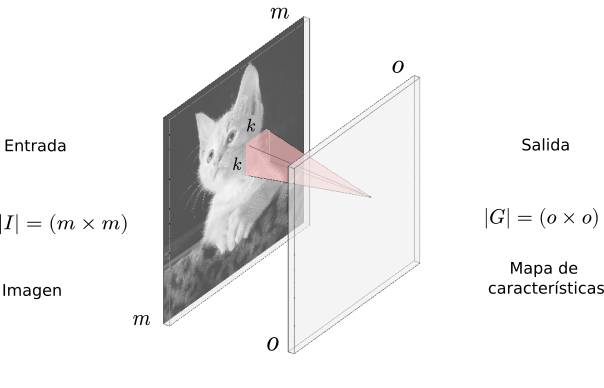
\includegraphics[height=0.7\textheight]{conv2d_es}
	\caption{Sizes of a 2D convolution}
	\label{fig:conv2des}
\end{figure}
\end{frame}


\begin{frame}
	\frametitle{Characterization}
	\begin{itemize}
		\item Output size
		\begin{equation}
			o = 1 + (m - \mathrm{k})
			\label{eq:output valid}
		\end{equation}
		\item Amount of parameters
		\begin{equation}
			| \theta | = \mathrm{k}_1 \cdot \mathrm{k}_2 + 1
		\end{equation} 
	\end{itemize}
\end{frame}



\section{Multichannel convolution}

\begin{frame}
\frametitle{Multichannel input}
	\begin{itemize}
		\item In the majority of cases the input to a convolution layer has more than one channel, e.g. RGB images.
	\end{itemize}
	\begin{figure}
		\centering
		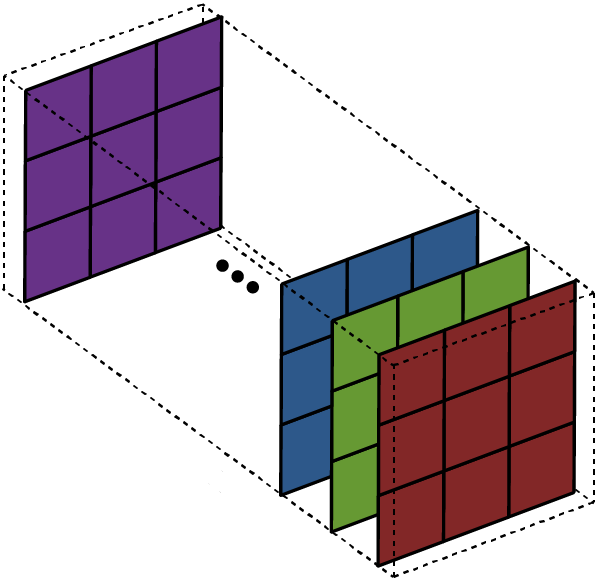
\includegraphics[height=0.6\textheight]{multichannel_input}
		\caption{Illustration of an input image with size $(c \times m \times m)$. $c$ indicates the number of channels.}
		\label{fig:markus-winkler-afw1hht0nss-unsplash}
	\end{figure}
\end{frame}


\begin{frame}
	\frametitle{Multichannel convolution}
	\begin{itemize}
		\item The kernel size is $(c \times k \times k)$
		\item The kernel's width and height are usually smaller than the input but the depth is the same than the input number of channels.
		\item Computation:
		\begin{equation}
			\texttt{Conv2DMulticanal}(K,I,b)[i,j] = b + \sum_{w=1}^{c} \sum_{u=-l}^{l} \sum_{v=-l}^{l} K[w, u, v] I[w, i+u, j+v]
			\label{eq:conv multicanal}
		\end{equation}
	\end{itemize}
\end{frame}



\begin{frame}{Multichannel convolution}
	\framesubtitle{Illustration}
\begin{figure}
\centering
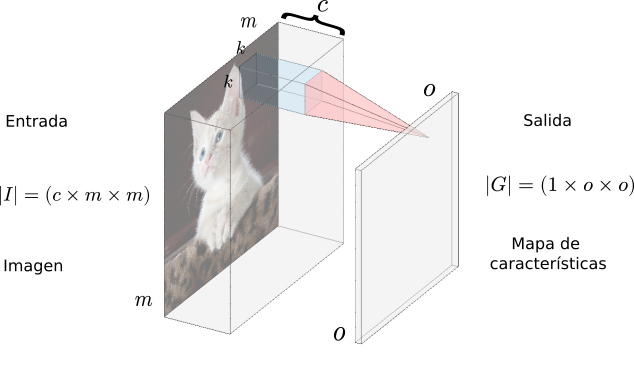
\includegraphics[height=0.7\textheight]{conv2d_multichannel_es}
\caption{Convolution sizes of the multichannel convolution. The kernel's width and height are usually smaller than the input but the depth is the same than the input number of channels}
\label{fig:conv2dmultichanneles}
\end{figure}
\end{frame}


%\begin{frame}
%\frametitle{CNN Convolution}
%\begin{figure}
%	\centering
%	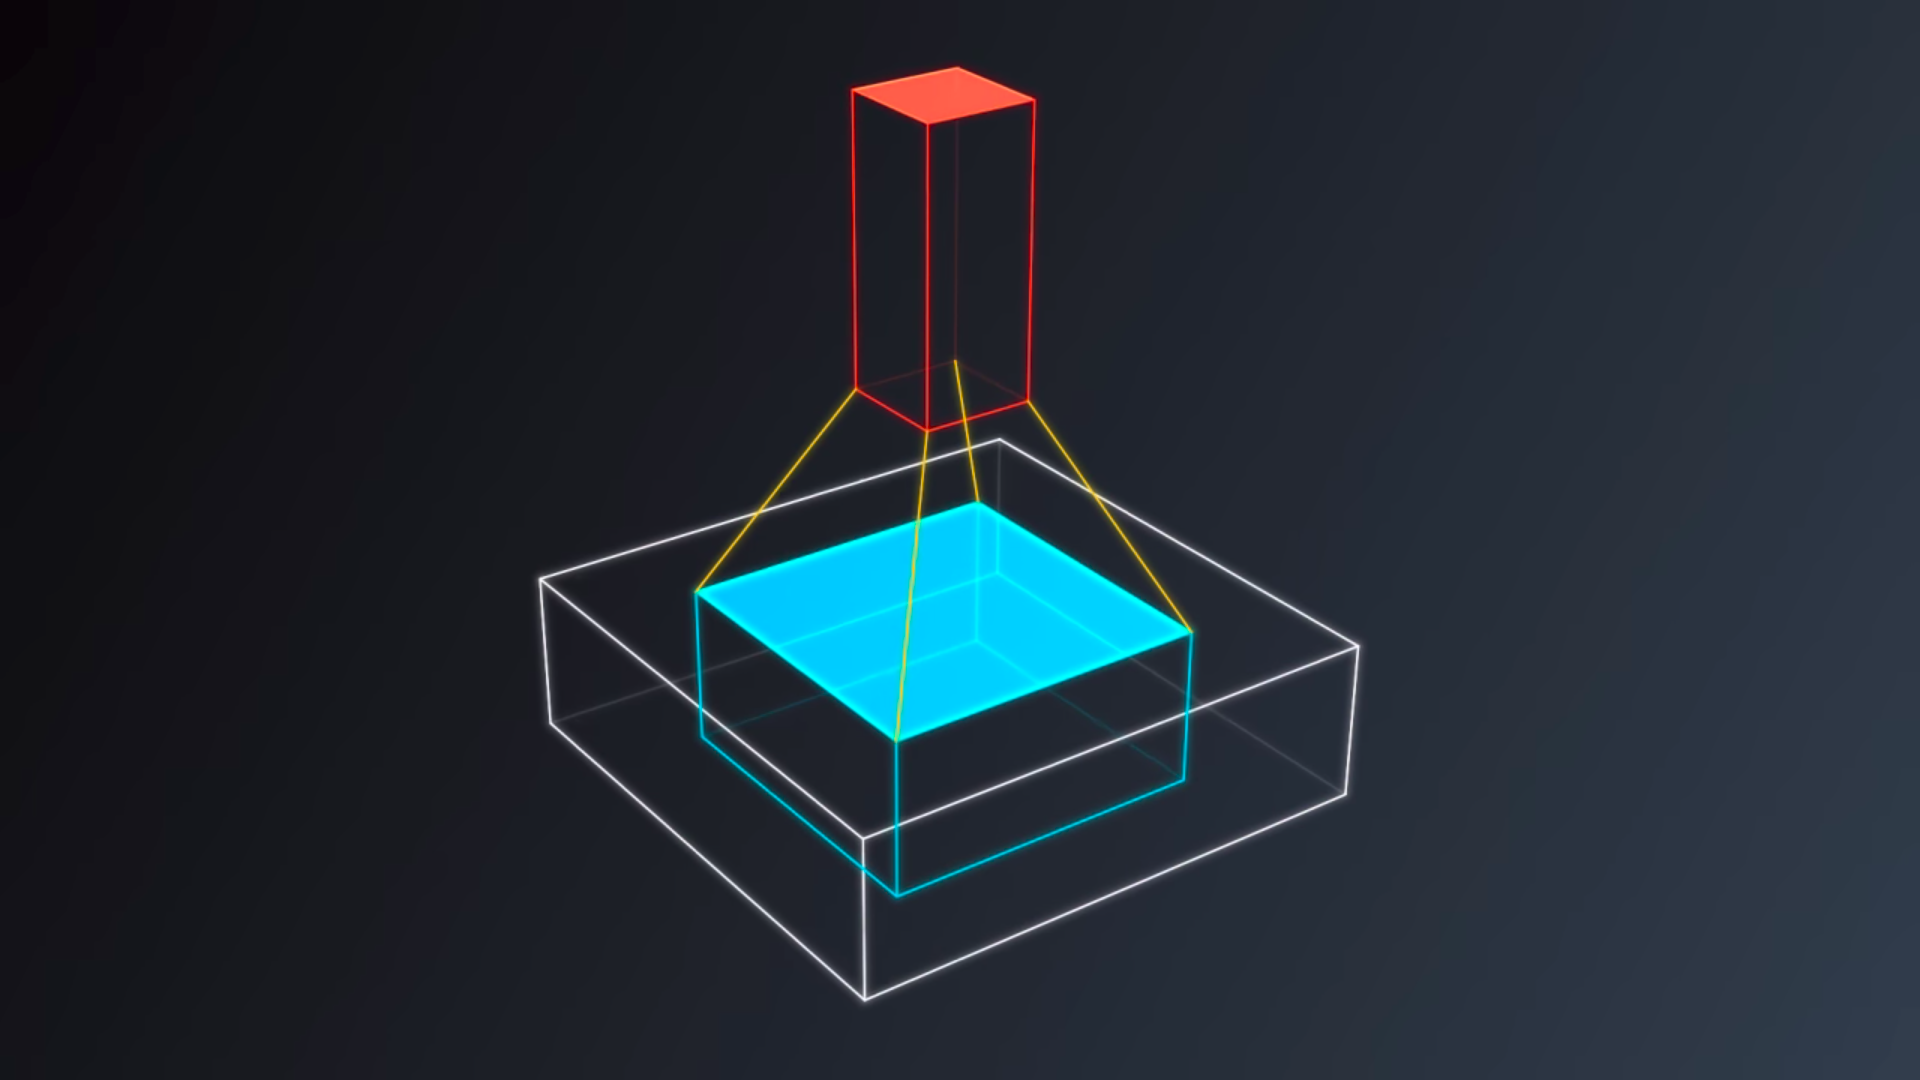
\includegraphics[width=\linewidth]{filter}
%	\caption{Convolution: a kernel is moved inside the input to create a new volume.}
%	\label{fig:filter}
%\end{figure}
%\end{frame}


\begin{frame}
	\frametitle{Multichannel convolution example}
\begin{figure}
	\centering
	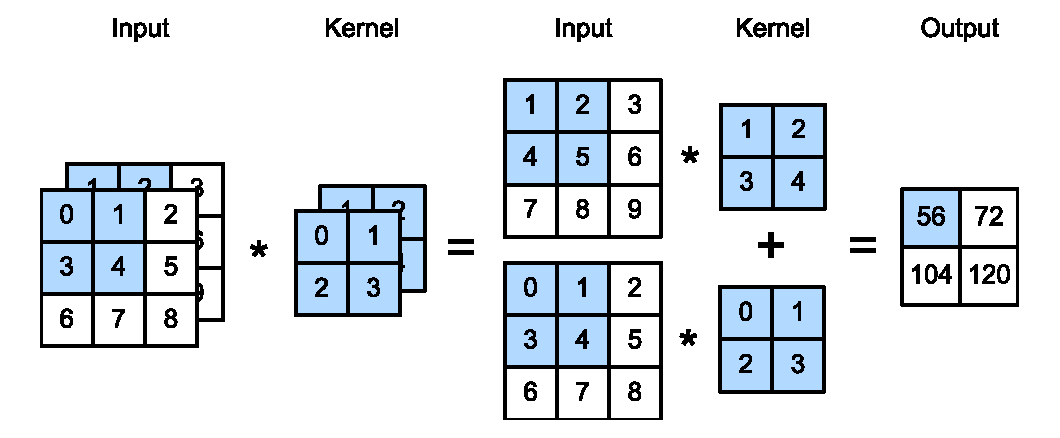
\includegraphics[height=0.7\textheight]{multichannel}
	\caption{}
	\label{fig:multichannel}
\end{figure}
\end{frame}



\section{Stride, padding and stacking}

\begin{frame}
\frametitle{CNN Stride}
\begin{figure}[tb]
	\centering
	% Cada subfigura ocupa ~1/4 del ancho del texto
	\begin{subfigure}[t]{0.24\textwidth}
		\centering
		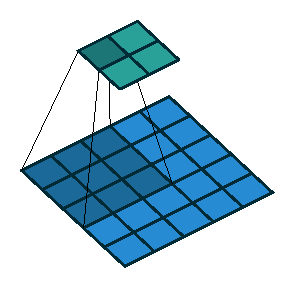
\includegraphics[width=\linewidth]{no_padding_strides_00.pdf}
		\caption{Subfig. 1}
		\label{fig:ejemplo:a}
	\end{subfigure}\hfill
	\begin{subfigure}[t]{0.24\textwidth}
		\centering
		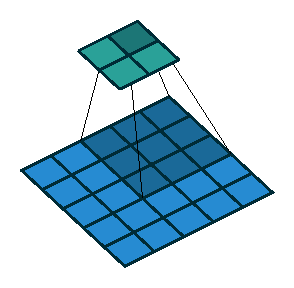
\includegraphics[width=\linewidth]{no_padding_strides_01.pdf}
		\caption{Subfig. 2}
		\label{fig:ejemplo:b}
	\end{subfigure}\hfill
	\begin{subfigure}[t]{0.24\textwidth}
		\centering
		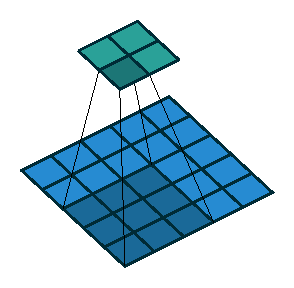
\includegraphics[width=\linewidth]{no_padding_strides_02.pdf}
		\caption{Subfig. 3}
		\label{fig:ejemplo:c}
	\end{subfigure}\hfill
	\begin{subfigure}[t]{0.24\textwidth}
		\centering
		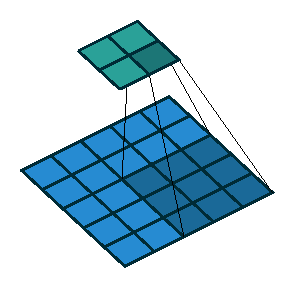
\includegraphics[width=\linewidth]{no_padding_strides_03.pdf}
		\caption{Subfig. 4}
		\label{fig:ejemplo:d}
	\end{subfigure}
	
	\caption{Visualización del proceso de convolución con salto $s=2$. El salto o \textit{stride} provoca un desplazamiento mayor del kernel.}
	\label{fig:convolucion_stride}
\end{figure}
\end{frame}

\begin{frame}
	\frametitle{CNN Stride (2)}
	\framesubtitle{output size}

	\begin{itemize}
		\item The stride is defined by $s$
		\item The output feature width size is then:
		\begin{equation}
			o = \lfloor \frac{i - k}{s} \rfloor + 1
		\end{equation} where $i$ is the input, $k$ the kernel size, $o$ is the output size,
		\item The same applies for height
	\end{itemize}
\end{frame}



\begin{frame}
\frametitle{CNN Padding}
\begin{itemize}
	\centering
	\item Valid padding:\\	
	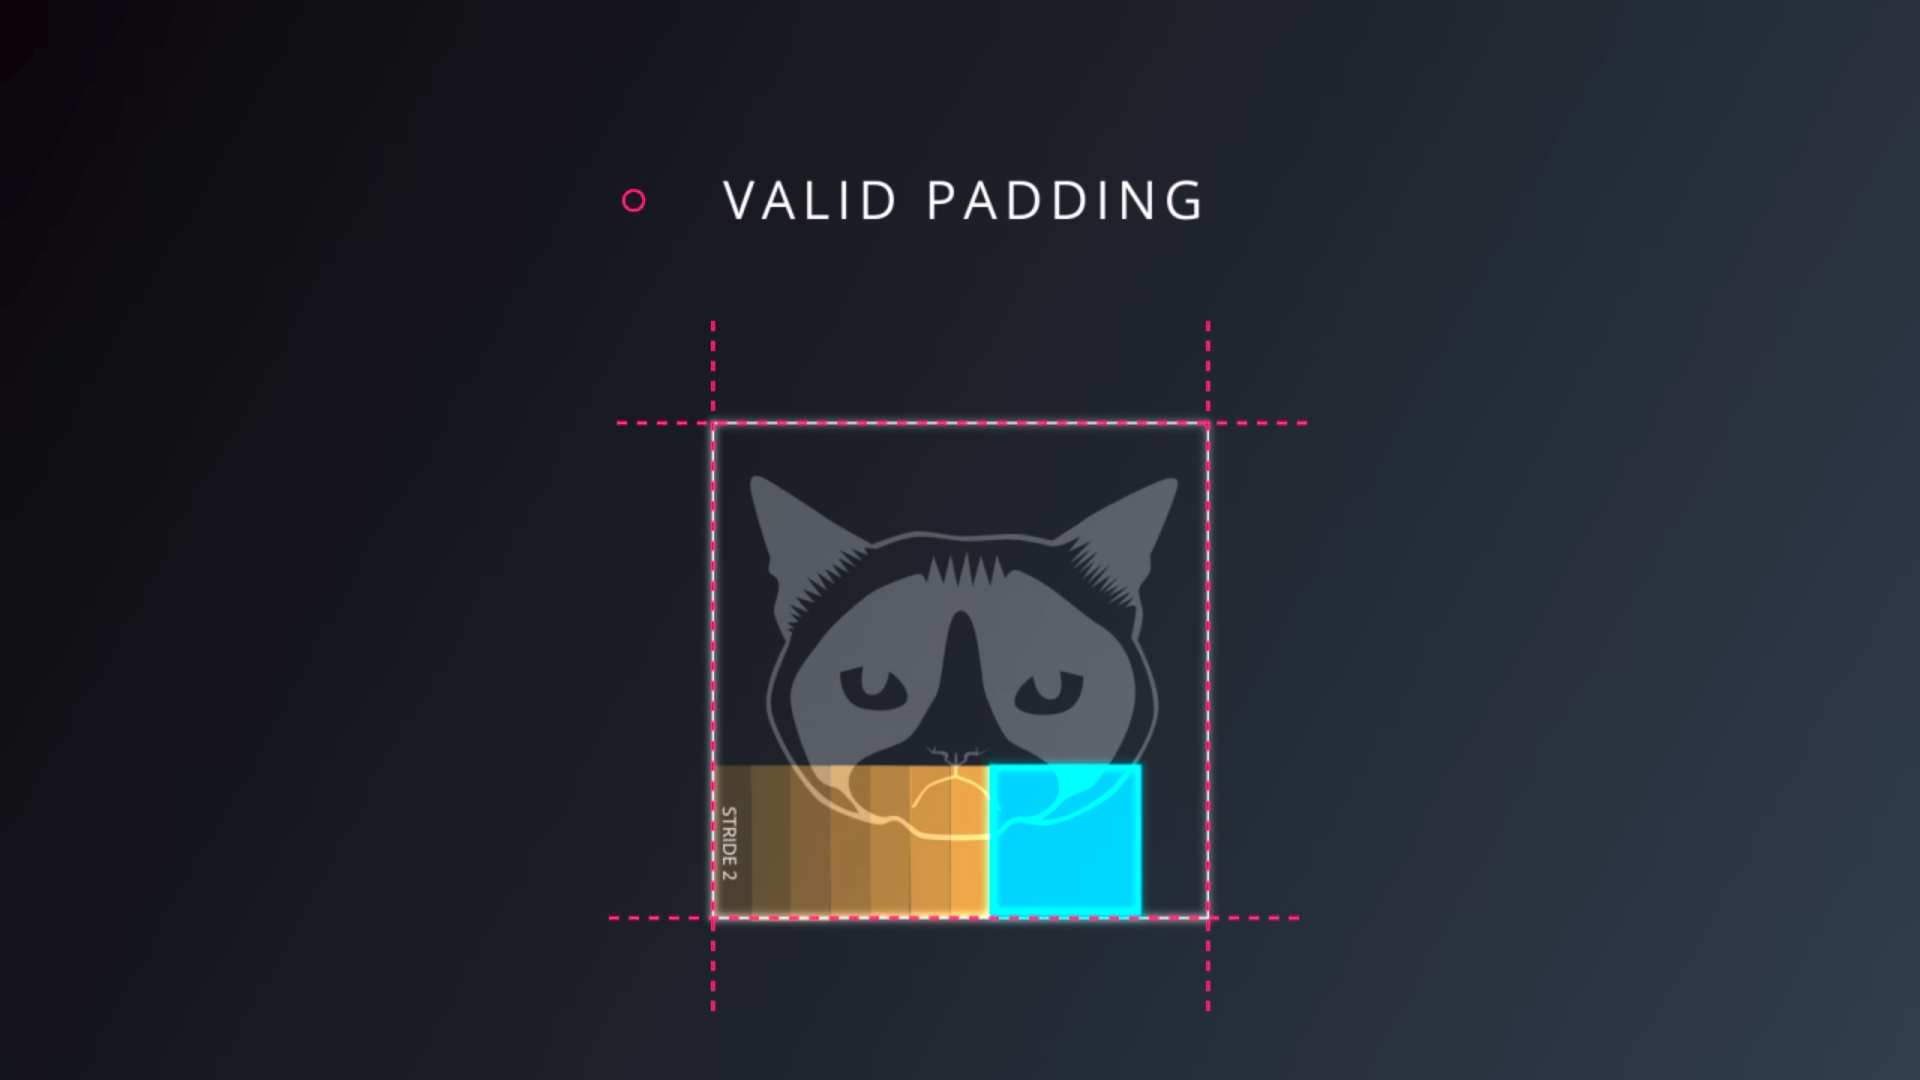
\includegraphics[trim={0 1cm 0 10cm}, clip, height=0.35\textheight]{valid}
	\item Same padding adds zeros\\
	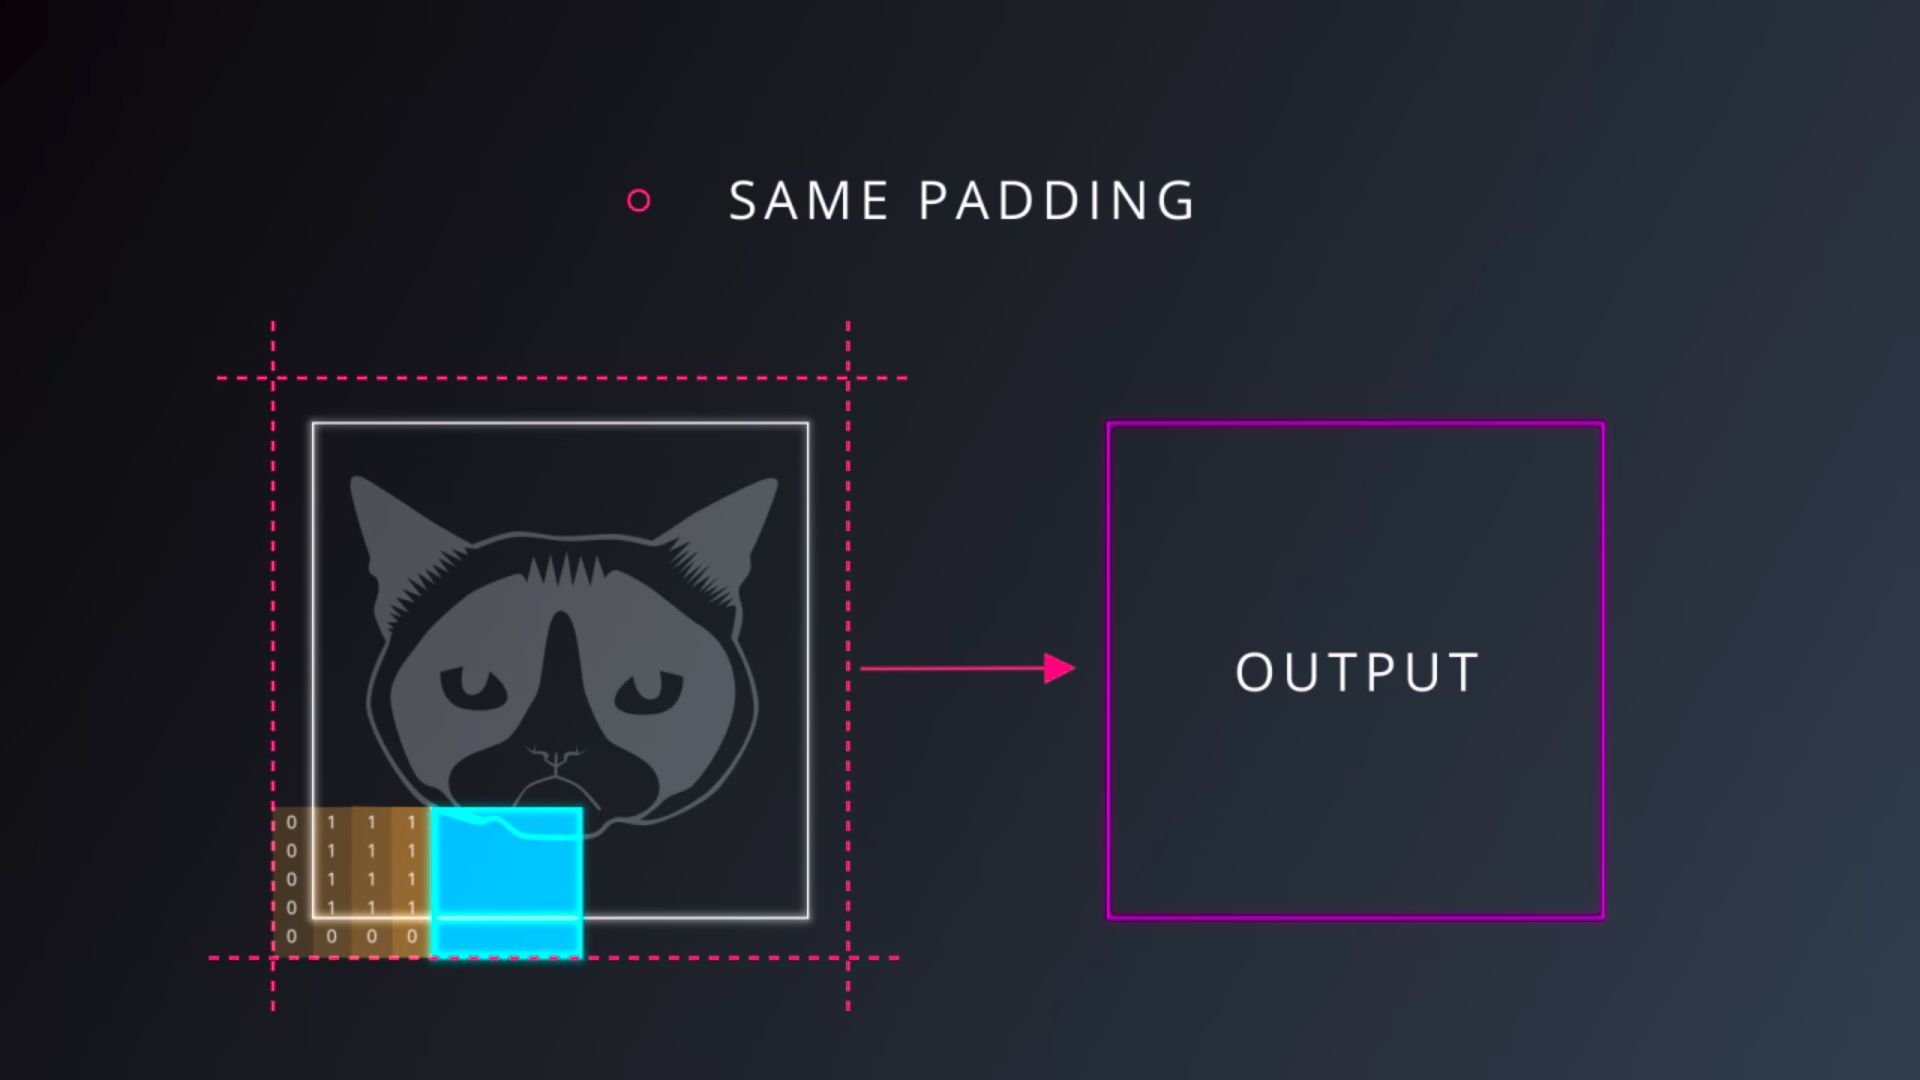
\includegraphics[trim={0 1cm 0 10cm}, clip, height=0.35\textheight]{same_padding}
\end{itemize}
\end{frame}


\begin{frame}
\frametitle{CNN Padding}
\framesubtitle{Padding output arithmetic}
For any $i$, $k$, $p$ and $s$:
\begin{equation}
	o = \lfloor \frac{i + 2p - k}{s} \rfloor + 1
\end{equation}
\end{frame}


\begin{frame}
	\frametitle{Convolution layer with several kernels}
	\begin{itemize}
		\item A convolutional layer can apply several kernels to the same input.
		\item The output of each convolution is stack in the feature map.
	\end{itemize}
	\begin{figure}
		\centering
		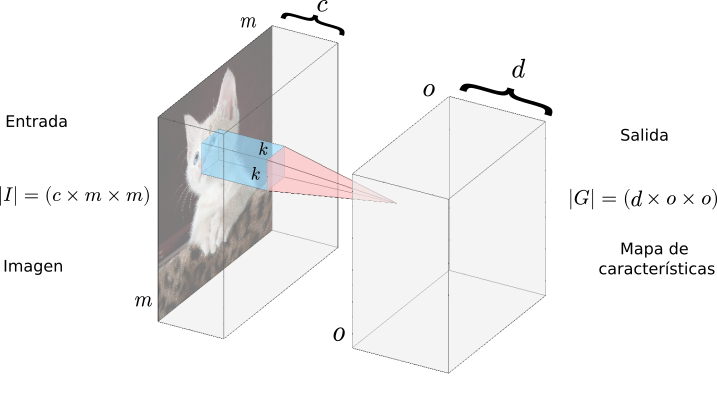
\includegraphics[height=0.65\textheight]{conv2d_stack}
		\caption{The depth of the feature map is the same as the number of applied kernels.}
		\label{fig:conv2dstack}
	\end{figure}
\end{frame}


\begin{frame}
\frametitle{Exercise}
\begin{itemize}
\item	Given: An input of $(3 \times 28 \times 28)$, 8 kernels of $(3 \times 3 \times 3)$, calculate the size of the feature maps:

\centering
\begin{tabular}{|c|c|c|c|c|c|}
	\hline 
	Padding & p & Stride (s) & Width & Height & Depth \\ 
	\hline 
	valid & 0 & 1 &  &  &  \\ 
	\hline 
	same & & 1 & 28 & 28 &  \\ 
	\hline 
	valid & 0 & 2 &  &  &  \\ 
	\hline 
\end{tabular} 
\end{itemize}
\end{frame}



\begin{frame}
\frametitle{Max Pooling}
\begin{figure}
	\centering
	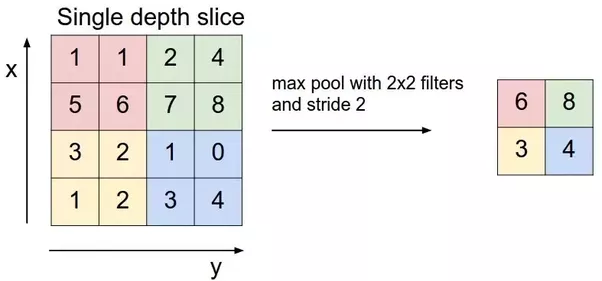
\includegraphics[height=0.6\textheight]{pooling}
	\caption{Pooling reduces the size of the feature map.}
	\label{fig:filter}
\end{figure}
\end{frame}

\begin{frame}
\frametitle{Pooling}
\begin{itemize}
\item Given $i$, $v$ and $s$, the output size is
\begin{equation}
	o = \lfloor \frac{i - v}{s} \rfloor + 1
\end{equation}
\item Some characteristics
\begin{itemize}
	\item Weights free
	\item A more accurate model
	\item Forward pass more expensive
	\item More hyper-parameters
\end{itemize}
\end{itemize}
\end{frame}


\begin{frame}
\frametitle{$1 \times 1$ convolution}
\begin{figure}
	\centering
	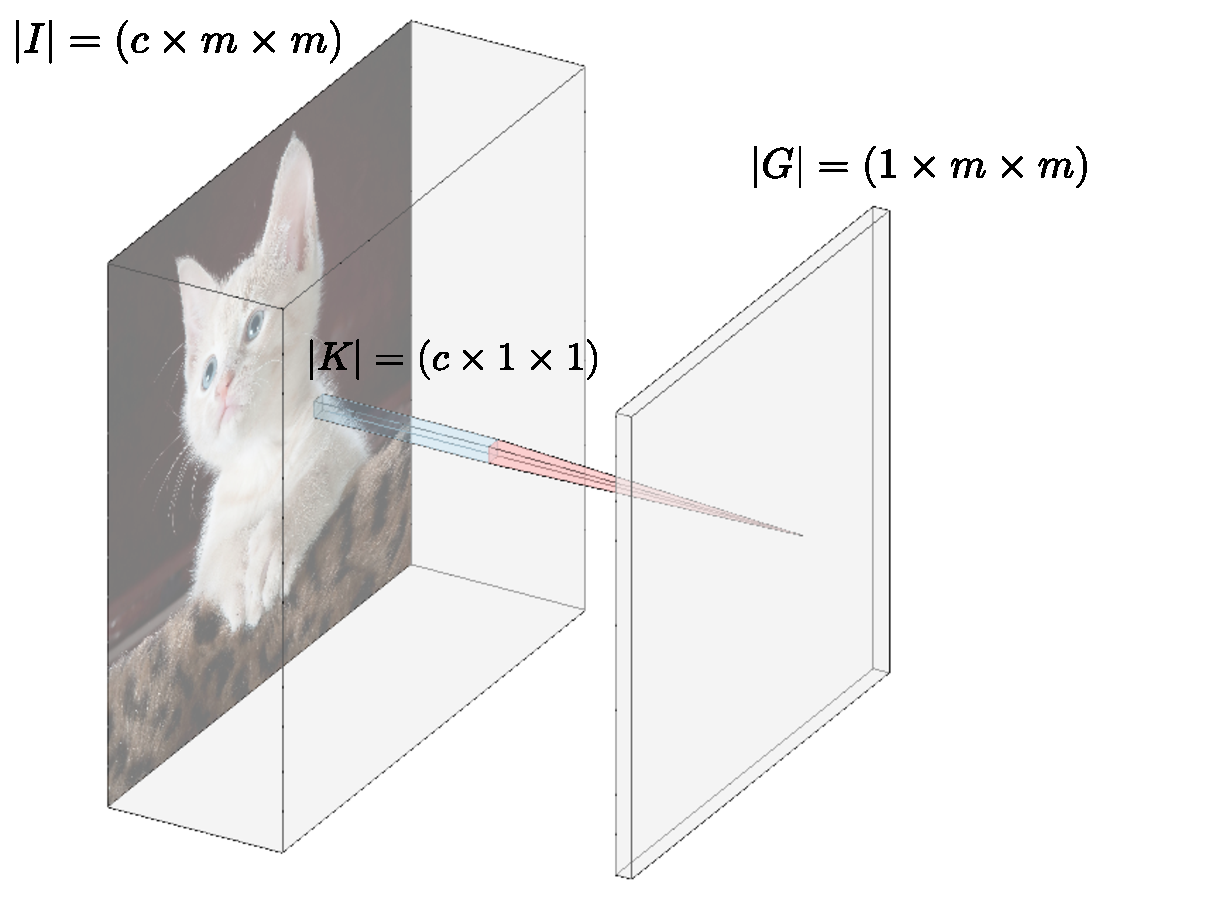
\includegraphics[height=0.7\textheight]{conv_1_1}
	\caption{A $1 \times 1$ convolution adds more parameters without modifying the structure.}
	\label{fig:filter}
\end{figure}
\end{frame}


\begin{frame}
\frametitle{Inception module (optional)}
\begin{figure}
	\centering
	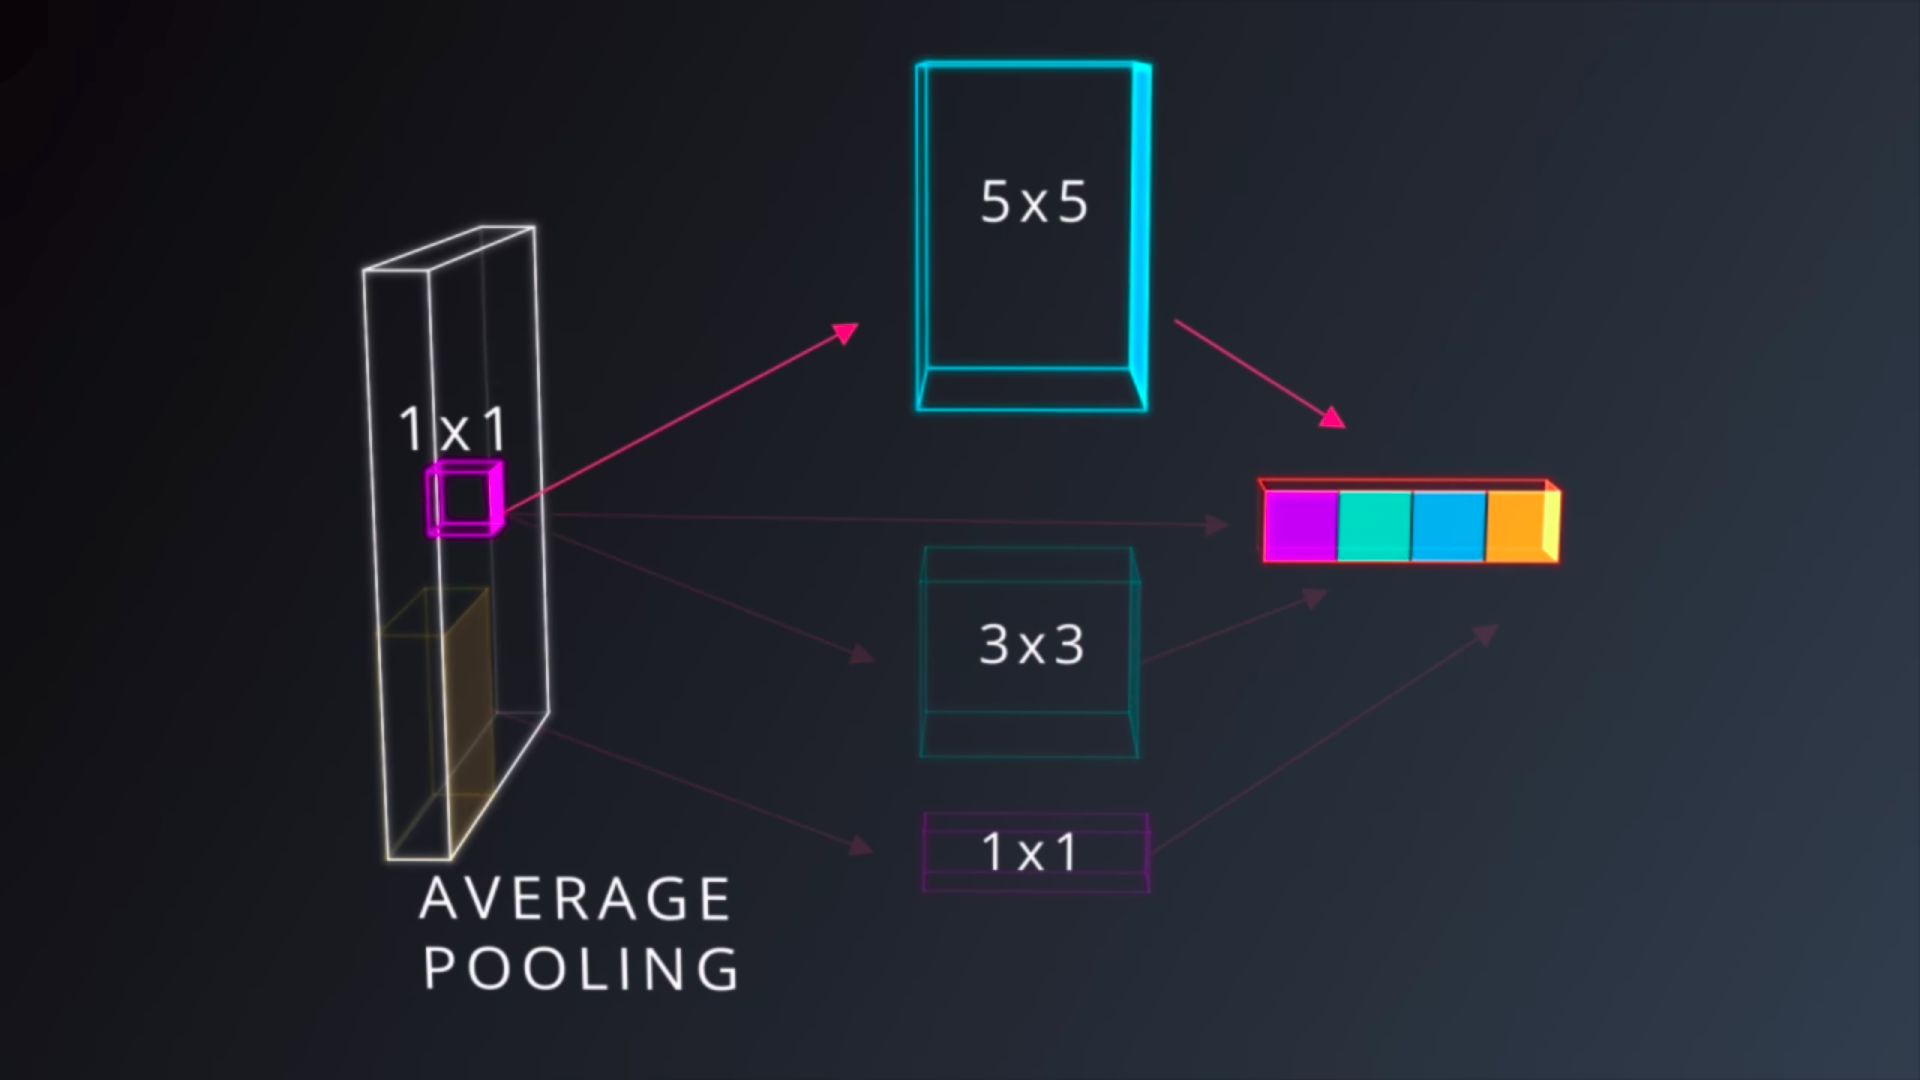
\includegraphics[height=0.6\textheight]{inception}
	\caption{Why to choose between different operations? Let make all!.}
	\label{fig:filter}
\end{figure}
\end{frame}


\begin{frame}
	\frametitle{CNN Classification}
	\begin{figure}
		\centering
		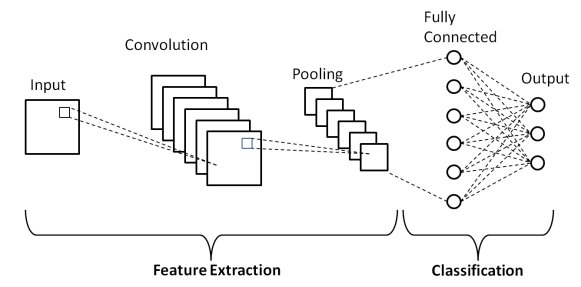
\includegraphics[height=0.6\textheight]{cnn scheme}
		\caption{In a CNN several convolutions are applied before a classification stage.}
		\label{fig:filter}
	\end{figure}
\end{frame}

\begin{frame}
	%\frametitle{CNN so far}
	\begin{figure}
		\centering
		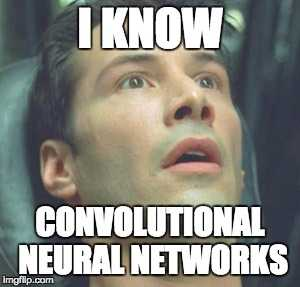
\includegraphics[height=0.9\textheight]{neo_convnets}
		%\caption{In a CNN several convolutions are applied before a classification stage.}
		%\label{fig:neo}
	\end{figure}
\end{frame}


\begin{frame}
\frametitle{References}
\begin{itemize}
	\item Dumoulin, Vincent, and Francesco Visin. "A guide to convolution arithmetic for deep learning." arXiv preprint arXiv:1603.07285 (2016).
	\item Juan Irving Vasquez, Introducción a las redes neuronales, Instituto Politécnico Nacional.
	\item Skansi, S. (2018). Introduction to Deep Learning: from logical calculus to artificial intelligence. Springer.
\end{itemize}
\end{frame}

\end{document}